
% 1. Start mit der Frage, wie RAG System Development in der Praxis abläuft. Vielleicht auch echte Praxiserfahrung mit reinnehmen (Blogs, etc.) -> Rekonfigurierbarkeit und Tuning soll sich herausstellen
% -> Grundlegende Frage für das Chapter Design: Wie kann man Rekonfigurierbarkeit und damit einhergehende reproduzierbaren, transparenten und sinnvollen Evaluation  in einer Umgebung für schnelles RAG Entwicklung sicherstellen?

% 2. RAG Entwicklung, welche Frameworks gibt es 
% -> Konfigurierbarkeit durch Files
% -> Maintainability
% -> Beliebtheit?
% -> Future Work (Haystack UI)
% -> Modularität (nach Gao.)
% -> IRA Methoden

% 3. Evaluation

% Genereller Blueprint Approach vorstellen

% 3.a)
% -> Warum sind beide Formen Comp und E2E wichtig?
% -> Was sind Herausforderungen ?
% -> Welche Frameworks für Evaluation gibt es?
% -> Für welches wurde sich entschieden, welche Metriken oder Objectives können sie einfangen?
% -> Wie wurden sie hier umgesetzt?

% 3.b)
% -> Wie kann ich Evaluierung truly Reproduzierbar und Transparent gestalten?
% -> Wichtige Frage ist vor allem wie können sie externe Valdität gewährleisten -> DAS WIRD DERZEIT IGNORIERT durch Overfitting-Tuning
% -> Was ist DVC und wird das gemacht?
% -> Welche Herausforderungen gibt es da?
% -> Welche Validity können gefährdet werden und welche können risiko-vermindert werden?

\section{External Validity of ML Experiments}

\begin{figure}
    \centering
    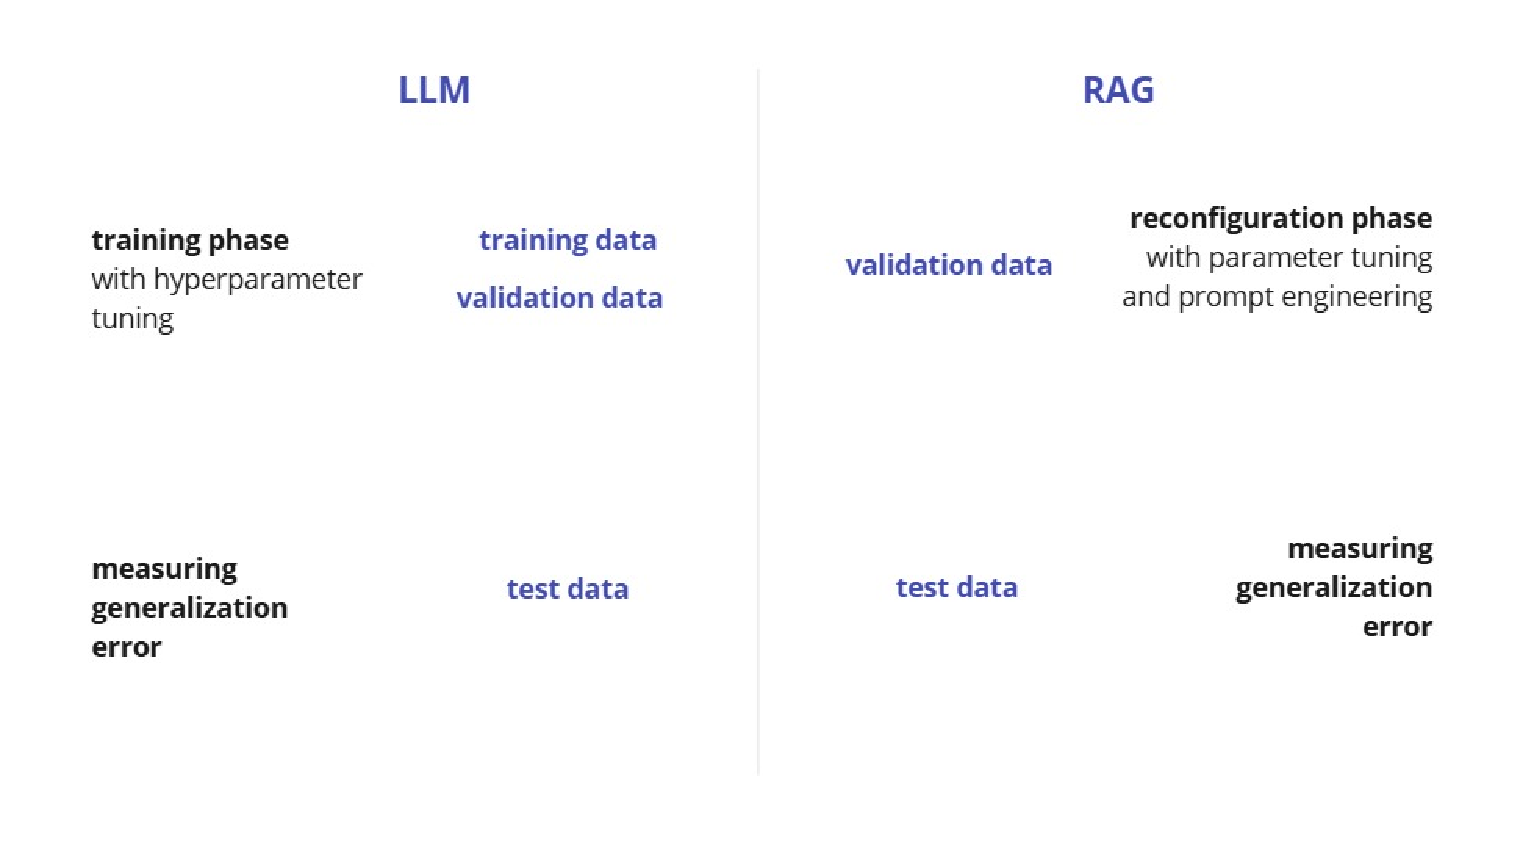
\includegraphics[width=\textwidth]{images/RAGvsLLM-tuning.pdf}
    \caption{Comparison of reconfiguration between RAGs and LLMs - both relying on tuning parameters and test data.}
    \label{fig:tuning}
\end{figure}


Developing retrieval-augmented generation systems is a difficult task that needs many reconfiguration phases, failure analytics and continous and rigorous testing.\cite{Simon.10112024,Barnett.2024,Ru.15.08.2024} Data is rare, especially for down-stream tasks in domains such as configuration validation or similar tasks. They often rely on few datasets that can not represent the whole domain. Therefore there are measures required to ensure that the developed systems can be generalized from the seen data to the unseen production data. Measuring generalization error in the large language model development is done by splitting the data into training, validation and test datasets. While the training and validation data is used for hyperparameter tuning to ensure the best performing model, the test dataset on the other hand is used to check if the hyperparameter tuning introduced an overfitting. This procedure must be adopted for RAG systems too (cf. figure \ref{fig:tuning}). Even though they do not rely on a training in the most cases, the continous reconfiguration of such systems, including prompt engineering or parameter tuning can lead to differences in seen and unseen data. The needs for a test dataset is independent from a potential training phase, but instead very dependent on a tuning phase for the systems, that is done till the results converge to the best outcoming scenario. Both LLM and RAG development share those reconfiguration phases.


\paragraph{External vs Internal Validity}

\paragraph{RAG Evaluation needs a Holdout-Testset}
\begin{itemize}
    \item RAG Experiments belongs to ML Experiments
    \item ML Experiments might cause Overfitting
    \item Generalization (External Validity) is testable with a hard data split (train vs validation vs test)
    \item training data split is not needed, but validation and test is required
    \item validation is for hyperparameter tuning important, which configs have the best results
    \item no testset -> no generalization estimatation
\end{itemize}

% referencing to Simon Paper

\begin{figure}[!ht]
    \centering
    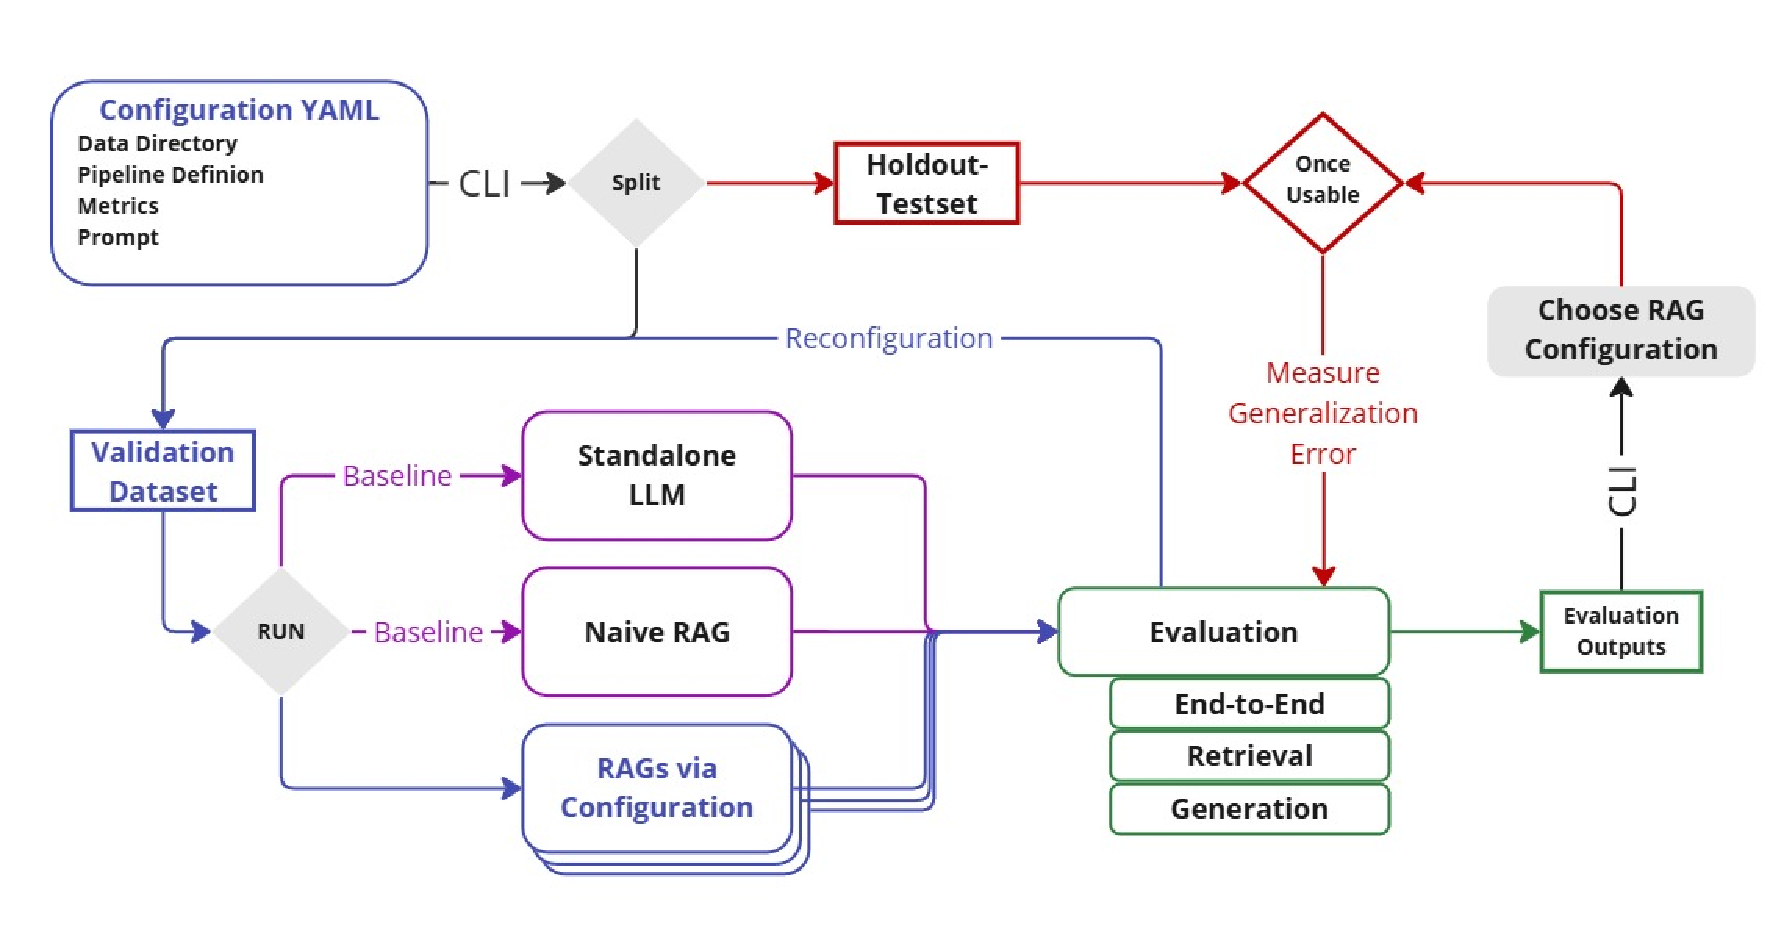
\includegraphics[width=\textwidth]{images/Sketch.pdf}
    \caption{...}
    \label{fig:EvaluationDesign}
\end{figure}


\section{Reproducibility of ML Experiments}
\begin{itemize}
    \item Seeding
    \item DVC 
    \item Logging all information
    \item Reporting
\end{itemize}

\section{Relevant Metrics for RAGs}
\begin{itemize}
    \item Task-specific vs Model-specific
    \item Performance vs System
    \item + Robust and Ethics
    \item Classification Metrics vs Generation Metrics
    \item RAGAS and Co. -> What do I need here?
\end{itemize}

\section{Coverage of Variety of RAG-Systems}

How I chose the right framework for it (Haystack vs Llama-Index vs Langchain)


